\setchapterstyle{kao}
\setchapterpreamble[u]{\margintoc}


\chapter{The IceCube Neutrino Observatory}
\labch{icecube}

\todo{add fancy icecube picture}

The IceCube Neutrino Observatory \sidecite[6cm]{2017JInst..12P3012A_Instrumentation_Systems} is a cubic-kilometer, ice-Cherenkov detector located at the geographic South Pole. IceCube utilizes the Antarctic glacial ice as detector medium to observe neutrinos by measuring the Cherenkov light produced from secondary charged particles with optical modules. It was deployed between 2006 and 2011 and has been taking data since the installation of the first modules. The primary goal of IceCube is the observation of astrophysical neutrinos as a telescope, but it can also be used to study fundamental particle physics properties by measuring atmospheric neutrinos as well as studying cosmic rays.

This chapter first describes the main- and sub-array of the detector and its detection module in \refsec{icecube_array}, the propagation of particles through ice is explained in \refsec{icecube_propagation}, and finally, the signatures that IceCube can observer of the different particles are introduced in \refsec{icecube_signatures}.


\section{IceCube Detector Components} \labsec{icecube_array}

\begin{figure}[h]
    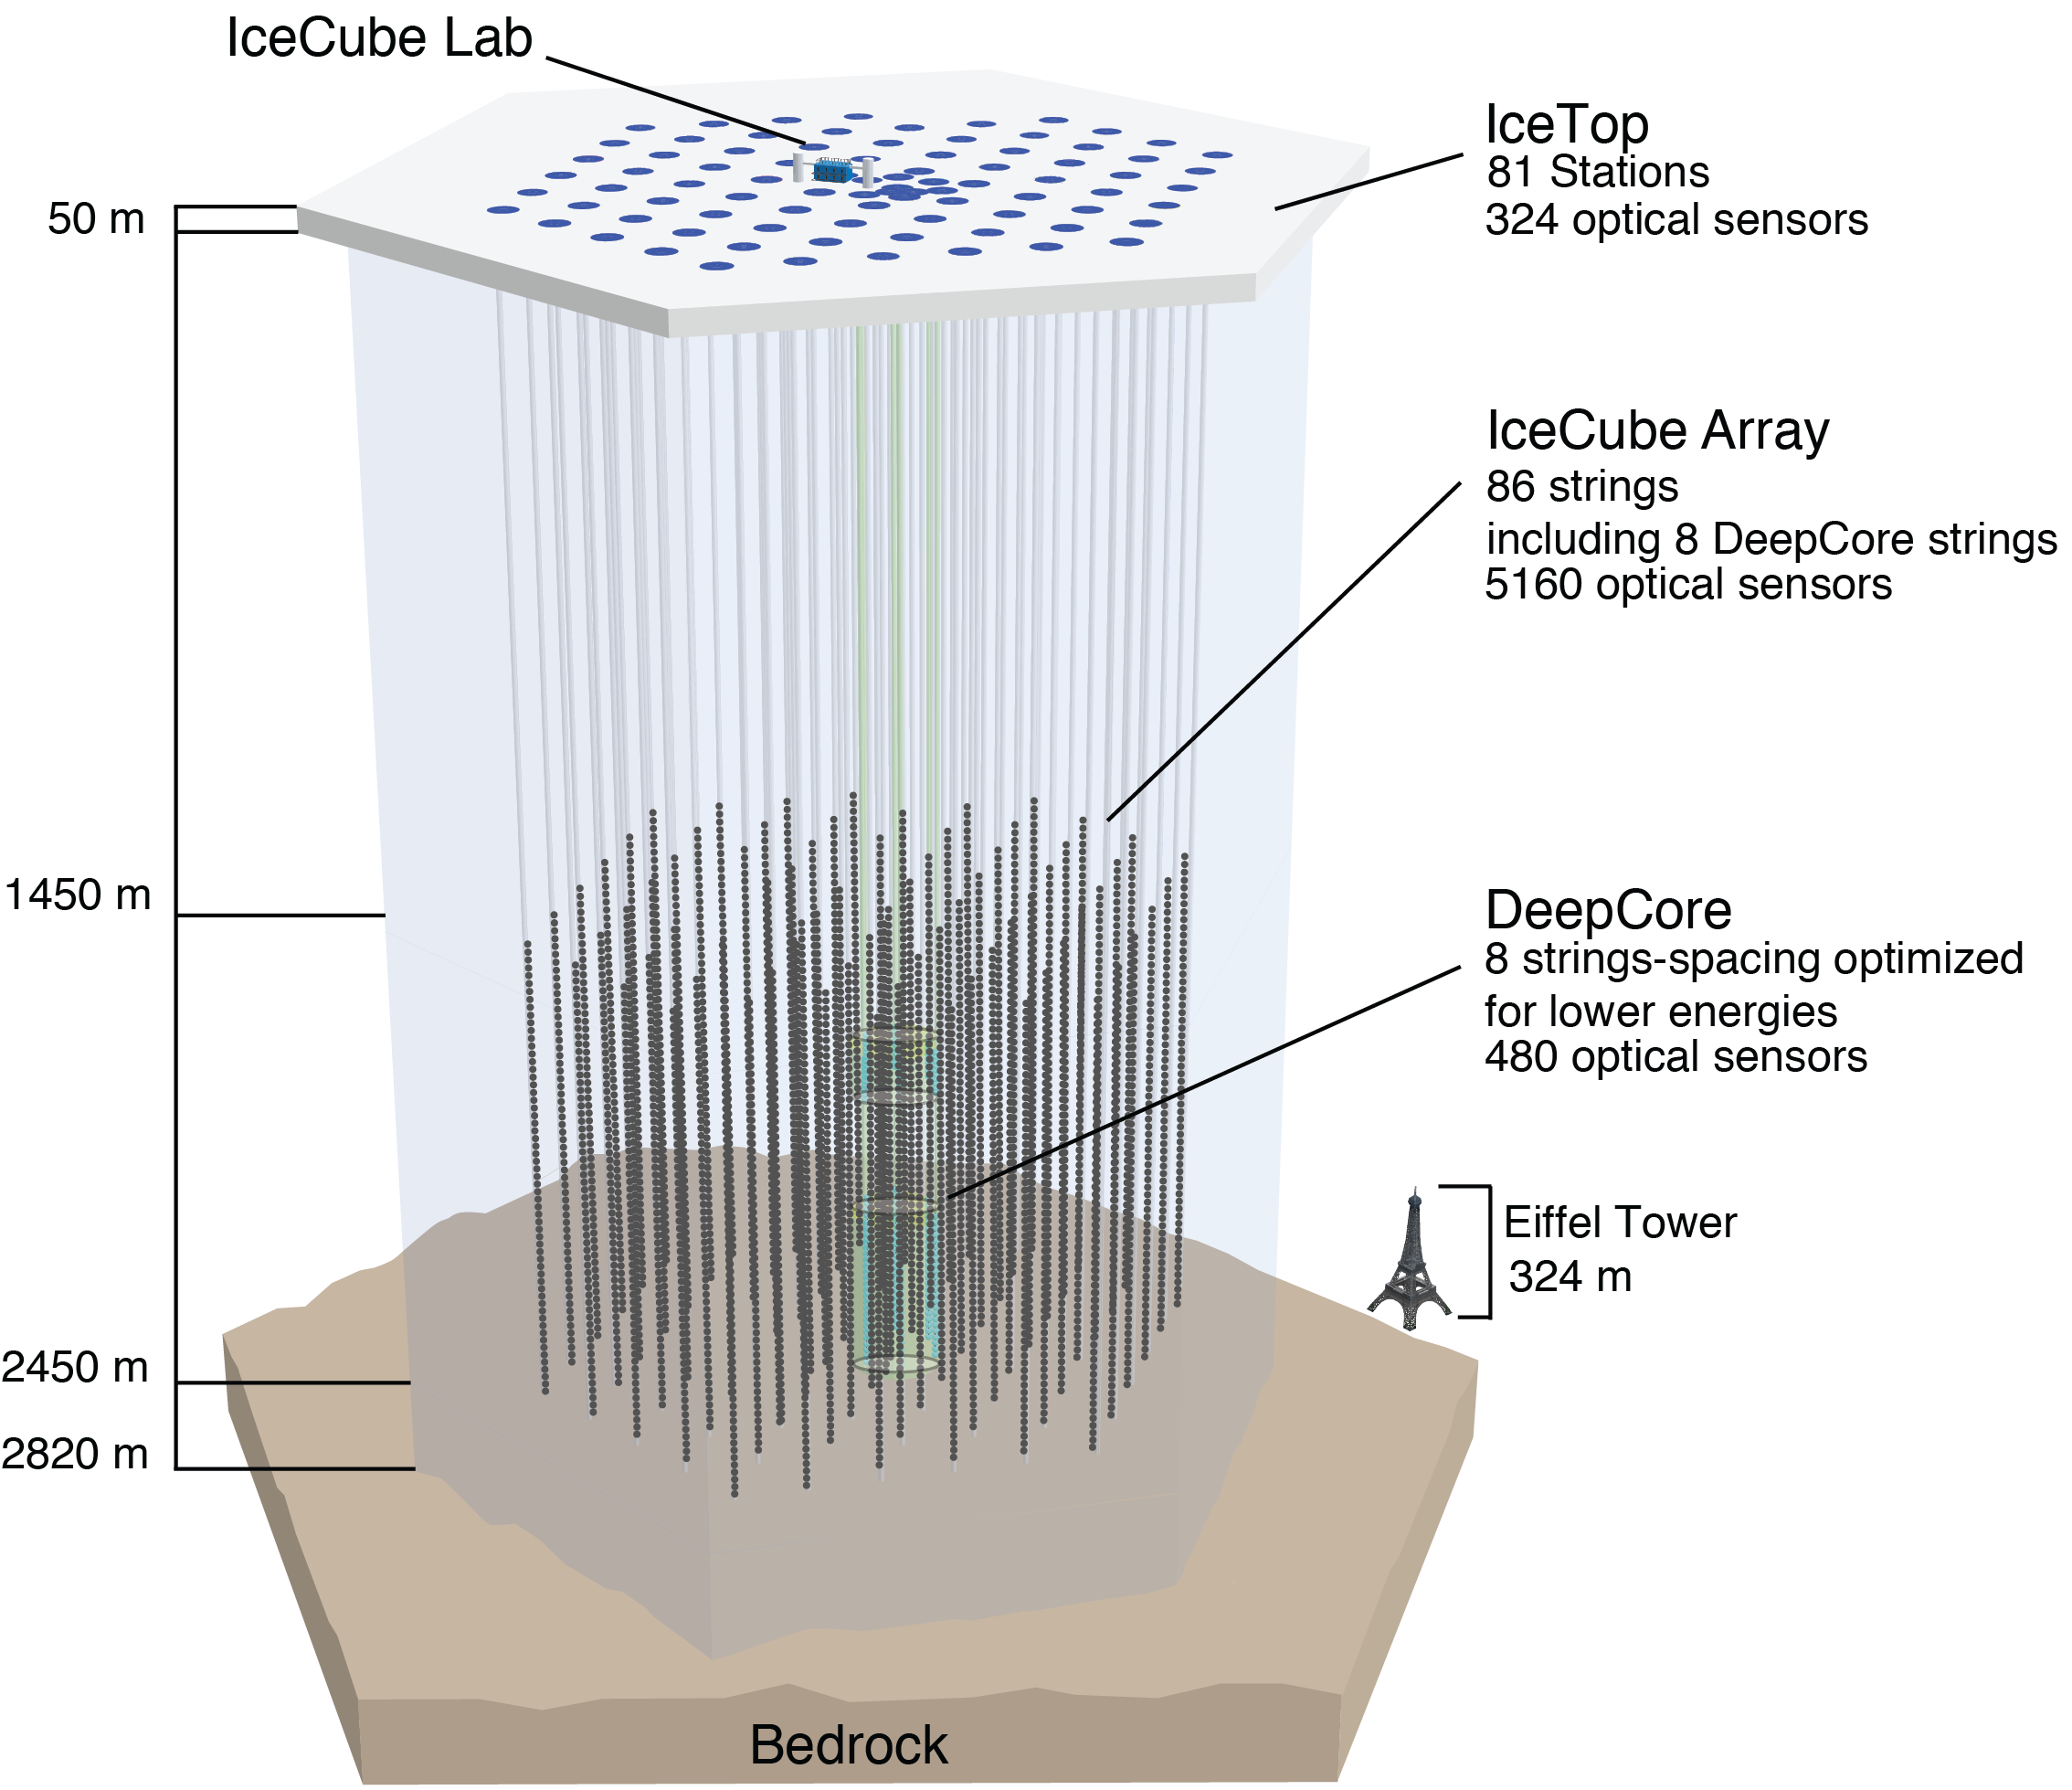
\includegraphics{figures/icecube_deepcore/IceCubeArray_slim.png}
	\caption[IceCube overview]{Overview of the IceCube detector showing the in-ice main- and sub-array IceCube and DeepCore, IceTop, and the IceCube Lab. From \cite{2017JInst..12P3012A_Instrumentation_Systems}.}
    \labfig{icecube_array}
\end{figure}

The full IceCube detector array consists of 86 vertical, in-ice strings and 81 surface stations as shown in \reffig{icecube_array}. The in-ice part is composed of 60 optical modules per string deployed at depths of \SIrange[range-phrase=-]{1450}{2450}{\metre} below the ice, while the surface stations of the comic air-shower array, \textit{IceTop}, are ice-filled tanks. The surface stations and the majority of the strings are arranged in a hexagonal grid with the operations building, the \textit{IceCube Laboratory} (ICL), central to the grid on the surface. A top view of the hexagonal arrangement is shown in \reffig{icecube_top_view}. The in-ice array is designed to detect neutrinos in the energy range from $\mathcal{O}$({GeV}) to $\mathcal{O}$(PeV).


\subsection{Digital Optical Modules and the Antarctic Ice} \labsec{ice_and_DOMs}

The IceCube detection medium is the Antarctic glacial ice, which was formed over \SI{100000}{years} by accumulation of snow that was subsequently compressed by its own weight to form a dense crystal structure \sidecite{glacial_ice}. As a result of this formation process, the optical properties, scattering and absorption, primarily change with depth. Within the detector volume the absorption length ranges from \SIrange[range-phrase=-]{100}{400}{\metre}, while the scattering length lies between \SIrange[range-phrase=-]{20}{100}{\metre}. They are correlated, with the absorption length being roughly four times the scattering length \sidecite{ice_calibration}. The vertical distribution of scattering and absorption length can be seen in \reffig{ic_dc_sidecut}, where one dominant feature is the \textit{dust layer} between \SIrange{2000}{2100}{\metre} depth. This region has a higher concentration of dust particles that where deposited in a period of high volcanic activity, which leads to bad optical properties in form of larger scattering and absorption.

\begin{figure}[h]
    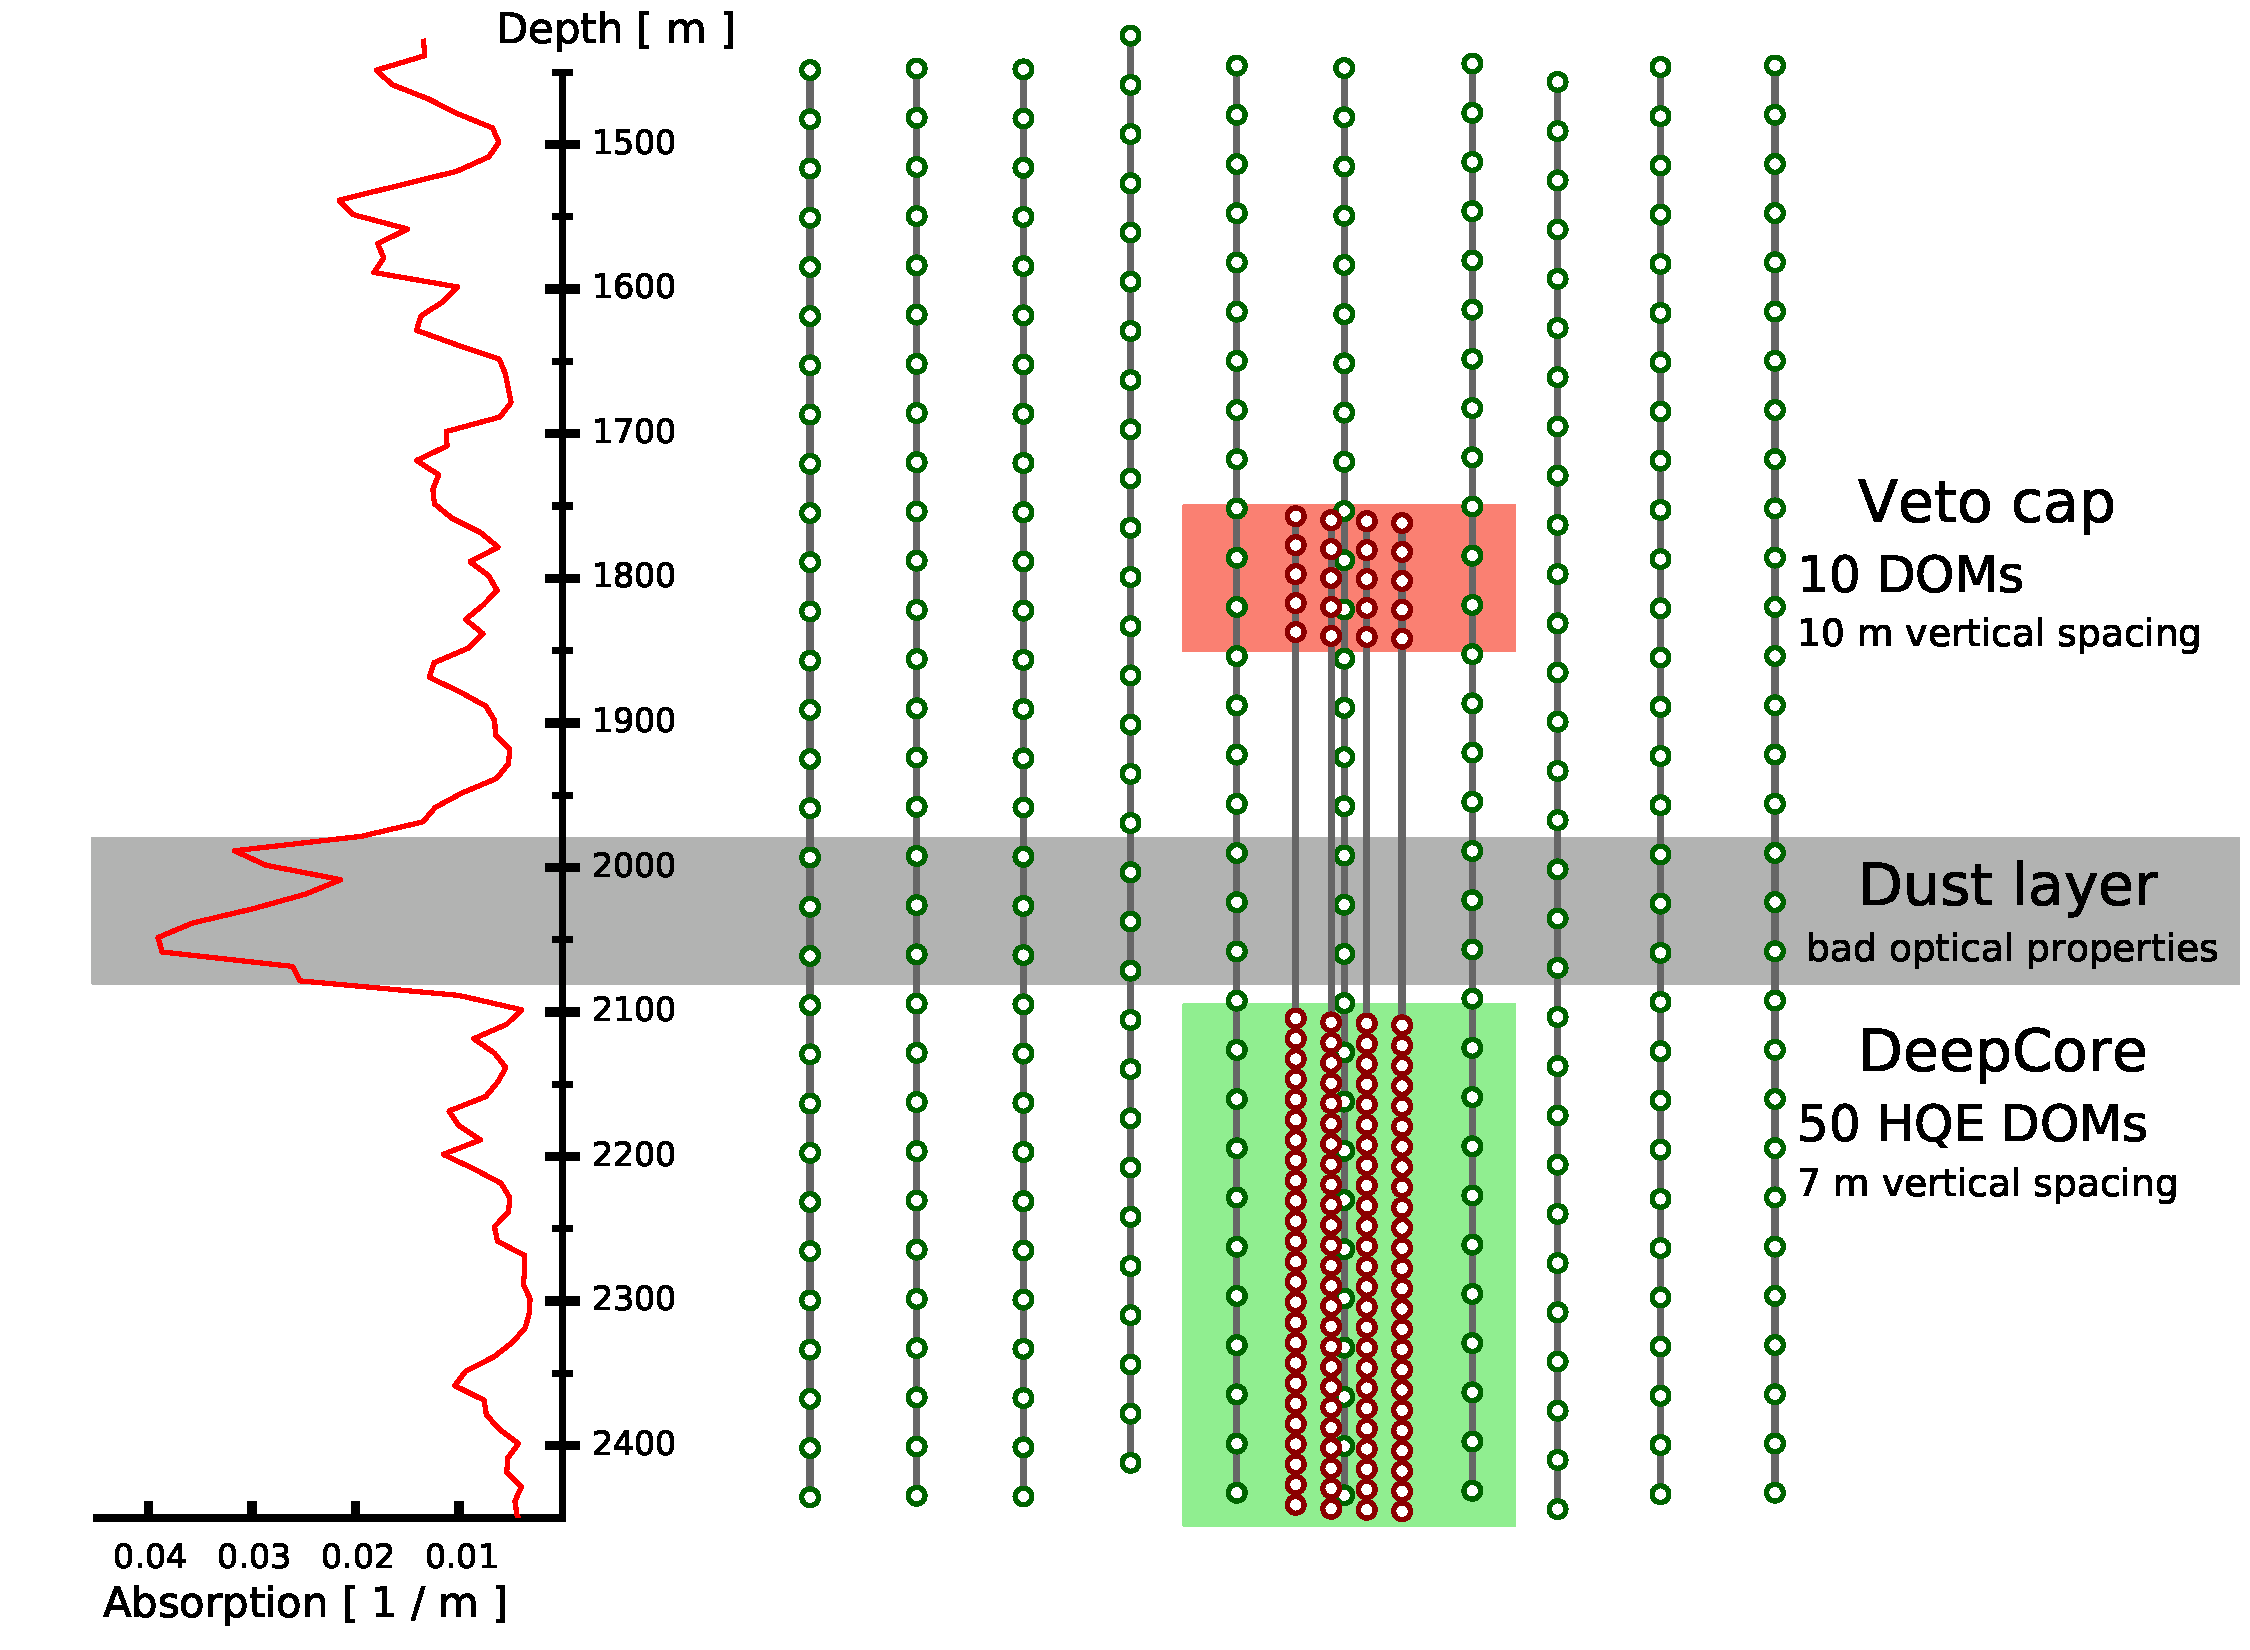
\includegraphics{figures/icecube_deepcore/DeepCore_sideview.pdf}
	\caption[IceCube sideview]{xx}
    \labfig{ic_dc_sidecut}
\end{figure}

\todo{exchange for figure with scattering (check abs/sca is cocrrect)}
\todo{mention/cite dust logger paper/procedure?}


The ice is instrumented by 5160 optical sensors called Digital Optical Modules (DOMs) \sidecite{ABBASI2009294_data_acquisition}, which can detect the Cherenkov light produced by charged particles traveling through the ice. Each DOM is made of a spherical glass housing, containing a downward-facing Photomultiplier Tube (PMT), the main board with control, readout, and processing-electronics, and a LED flasher board for calibration purposes. The design and the individual components of a DOM can be seen in \reffig{DOM_design}.

The majority of PMTs are the \SI{10}{"} Hamamatsu R7081-02, which have a bialkali photocathode and are sensitive to wavelengths in the range of \SIrange{300}{650}{\nano\metre}, with a peak quantum efficiency (quantum efficiency  of 25\% at \SI{390}{\nano\metre}. In the central part of the IceCube array the peak efficiency reaches 34\%. The dark count rate in the temperature range of \SIrange{-40}{-20}{\degreeCelsius} is $\sim$\SI{300}{\hertz}. The DOM electronics measure the PMT voltage and control the gain. At a voltage crossing of the equivalent to \SI{0.25}{PE} the waveform readout is activated \sidecite{ABBASI2009294_data_acquisition}. Only when either one of the nearest or next to nearest DOMs above or below also saw a voltage crossing within a \SI{1}{\micro\second} time window \sidenote{This is referred to as a \textit{hard local coincidence (HLC)}.}, the voltages are digitized and send to the ICL. Through the application of a waveform unfolding algorithm, called \textit{WaveDeform} \sidecite{IceCube:2013dkx}, the waveforms are compressed and the results are the reconstructed times and charges of the photo-electrons. This is the basis for all further IceCube data processing.

\begin{marginfigure}
    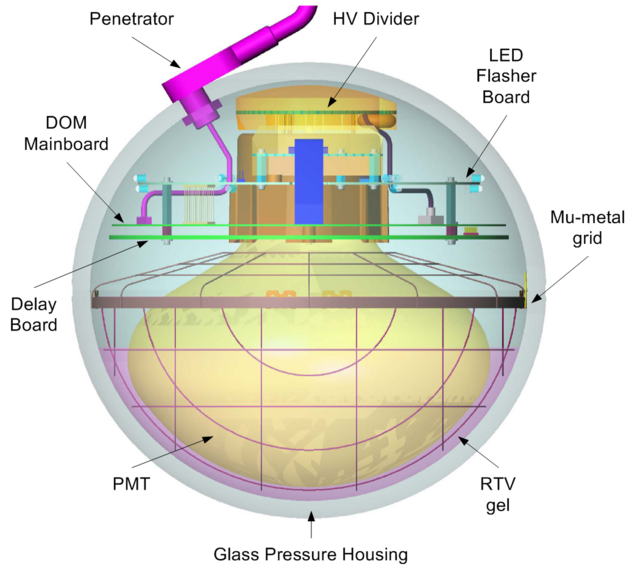
\includegraphics{figures/icecube_deepcore/DOM_schematic.png}
	\caption[Digital Optical Module (DOM)]{Design and components of a Digital Optical Module (DOM) \cite{ABBASI2009294_data_acquisition}}
    \labfig{DOM_design}
\end{marginfigure}

The PMT is covered with a mu-metal grid (made from wire mesh), shielding the photocathode from Earth's magnetic field and it is optically coupled to the glass sphere by RTV silicone gel. The glass sphere is a pressure vessel, designed to withstand both the constant ice pressure and the temporary pressure during the refreezing process of the water in the drill hole during deployment (peaking at around \SI{690}{\bar}). The sphere is held by a harness that connects the DOMs along a string and also guides the cable beside them.

The flasher board controls 12 LEDs that produce optical pulses in bright UV. The LEDs can be pulsed separately or in combination with variable output levels and pulse lengths. Using the known information of the light source positions and times this can be used for in-situ calibration of the detector by measuring absorption and scattering properties of the ice. Calibrating the optical efficiency of the DOMs itself is more accurately done using minimum ionizing muons \sidecite{domeff_nick}, since the total amplitude of the LED light is not well known.


\subsection{IceCube}

The 78 strings that are arranged in a hexagonal pattern from the main part of the in-ice array, which is called \textit{IceCube}. With a $\sim$\SI{125}{\metre} horizontal spacing between the strings and a $\sim$\SI{17}{\metre} vertical spacing between DOMs, IceCube has a lower energy threshold of around \SI{100}{GeV}. IceCube was designed to detect astrophysical neutrinos with energies above \SI{1}{\tera\electronvolt}.

The coordinate system that is used in IceCube is centered at 46500'E, 52200'N at an elevation of \SI{883.9}{\metre} \sidecite{2017JInst..12P3012A_Instrumentation_Systems}. Per definition, it's a right-handed coordinate system where the y-axis points along the Prime Meridian (Grid North) towards Greenwich, UK, and the x-axis points \SI{90}{\degree} clockwise from the y-axis (Grid East). The z-axis is normal to the ice surface, pointing upwards. For IceCube analyses depth is defined as the distance along the z axis from the ice surface, assumed to be at an elevation of \SI{2832}{\metre}.

\begin{figure}
    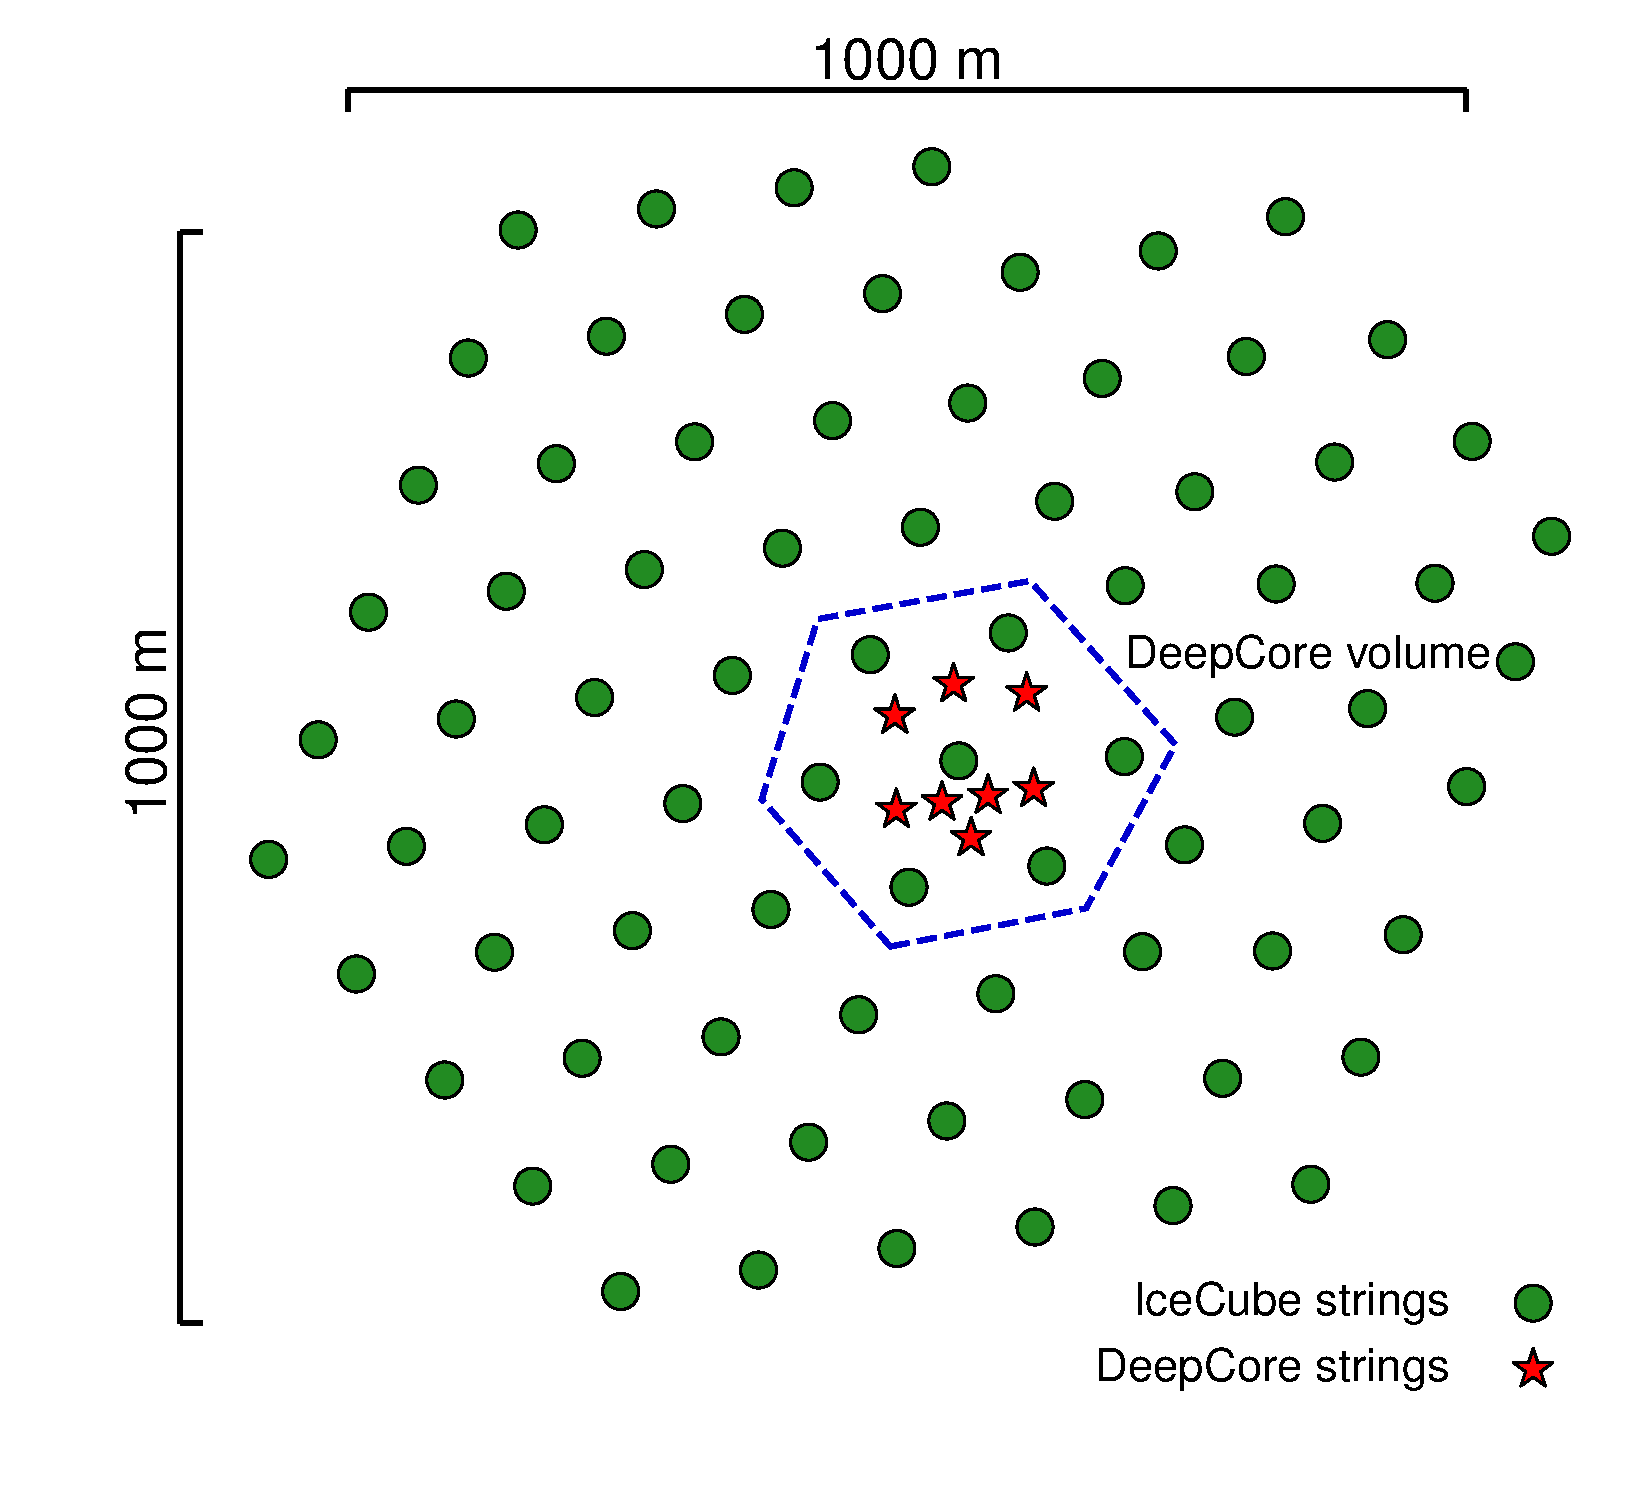
\includegraphics[trim={2.0cm, 1.5cm, 0, 0}, clip, width=0.65\linewidth]{figures/icecube_deepcore/icecube_top_view_bw.pdf}
    \caption[IceCube top view]{Top view of the IceCube array.}
    \labfig{icecube_top_view}
\end{figure}


\subsection{DeepCore}

The additional 8 strings form a denser sub-array of IceCube called \textit{DeepCore} \sidecite{DeepCore_design_Abbasi2012615}. It's located at the bottom-center of the in-ice array and its \textit{fiducial volume} also includes the 7 surrounding IceCube strings as shown in \reffig{icecube_top_view}. The strings in this region have a closer average horizontal distance of about \SI{70}{\metre}. Th lower 50 DeepCore DOMs on each string are placed in the region of clear ice below the dust layer between \SIrange{2100}{2450}{\metre} depth, where their vertical spacing is $\sim$\SI{7}{\metre}. The remaining 10 modules on each string are placed above the dust layer to be used as veto against atmospheric muons. Additionally, the DeepCore DOMs are equipped with higher quantum efficiency PMTs. The combination of the denser spacing and the high quantum efficiency modules, leads to a lower energy detection threshold of around \SI{5}{GeV}, allowing the observation of atmospheric neutrinos, which are mostly in the energy range of \SIrange{10}{100}{\giga\electronvolt}. The main analysis performed with DeepCore is an atmospheric neutrino oscillation measurement, but the large flux of atmospheric neutrinos allows for many other Beyond Standard Model searches, such as searches for dark matter, non-standard interactions, or sterile neutrinos. 


\section{Propagation of Particles in Ice} \labsec{icecube_propagation}


\todo{(Re-)write introduction for PhD thesis (just copy paste from M.Sc.). (everything below)}

When charged particles travel through matter they interact and lose energy by several interaction processes.
The Cherenkov light emitted by the particles as described in Section \refsec{cherenkov_effect} only contributes a small amount to the total energy loss.
The dominant processes depend on the type of Cherenkov light source, which we can broadly categorize into the three groups: quasi-continuous energy loss by muons, electromagnetic cascades, and hadronic cascades.

\paragraph{Muons} lose their energy mainly by \textit{ionization}, \textit{bremsstrahlung}, \textit{pair production} and the \textit{photo-nuclear interaction}.
Considering that ionization only has a weak energy dependence for muons above 1\,GeV and combining the other three components into one, the total energy loss is given by
\begin{equation}
    -\frac{\mathrm{d}E}{\mathrm{d}x} = a_I(E) + b_R(E) \cdot E,
    \labeq{radiative_losses}
\end{equation}
where $E$ is the energy and $a_I(E)$ and $b_R(E) \cdot E$ are the energy loss by ionization and the combined radiative losses, respectively.
For the energy range of interest for this work, the parameters $a_I(E)$ and $b_R(E)$ only have a weak energy dependence and equation \refeq{radiative_losses} reduces to
\begin{equation}
    -\frac{\mathrm{d}E}{\mathrm{d}x} = a + b \cdot E.
    \labeq{radiative_losses_simple}
\end{equation}
This description results in a critical energy $E_{crit}=a/b$ separating the two energy regimes where ionization or radiative losses are dominant.
Typical values are $a \approx 2.59$\,MeV/cm and $b \approx 3.63 \cdot 10^{-6}$\,cm$^{-1}$ \sidecite{2004hep.ph....7075C} leading to a critical energy of $\sim 770$\,GeV.
Since the considered energy range for atmospheric neutrino oscillations is below the critical energy we only consider ionization losses by setting $b=0$ which easily relates the range of a muon $R_\mu$ to its initial energy by
\begin{equation}
    R = \frac{E_0}{a}.
    \labeq{muon_range_approx}
\end{equation}
With equation \refeq{muon_range_approx} it is clear that by measuring the length of a muon track, its energy can be estimated if the full track is contained in IceCube.
This treatment is only an approximation and does not take into account the stochastic nature of some of the energy losses.
Especially bremsstrahlung and photo-nuclear interactions occur rarely, but when they happen, they deposit a large amount of energy. More detailed information is found in \sidecite{LRaedel}.


\subsection{Cherenkov Effect} \labsec{cherenkov_effect}

Cherenkov radiation is emitted when a charged particle moves through a medium with a velocity that is greater than the speed of light in that medium.
The continuous energy loss due to the emission of Cherenkov radiation is small, at the order of $\mathcal{O}$($10^{-4}$), as compared to the main energy losses that will be described in Section \refsec{energy_loss}.
The observation of this radiation in IceCube and DeepCore, however, is fundamental for the detection of the charged particles originating from the neutrino interactions that were outlined in Section \refsec{neutrino_interactions}.
The Cherenkov effect was first observed by Pavel Cherenkov in 1934 \sidecite{CherenkovPhysRev.52.378}.
As can be derived from trigonometry, the Cherenkov light is emitted in a parallel wavefront at the Cherenkov angle
\begin{equation}
    \theta_c = \arccos\Big(\frac{1}{\beta n}\Big),
    \labeq{cherenkov_angle}
\end{equation}
with $n$ being the refractive index of the medium and $\beta$ the speed of the particle in units of the speed of light.
A sketch of the wavefront is shown in Figure \reffig{cherenkov_light_front}, where the black circles depict spherically emitted light and the blue line is the formed Cherenkov light front.
\begin{figure}[h]
    \centering
    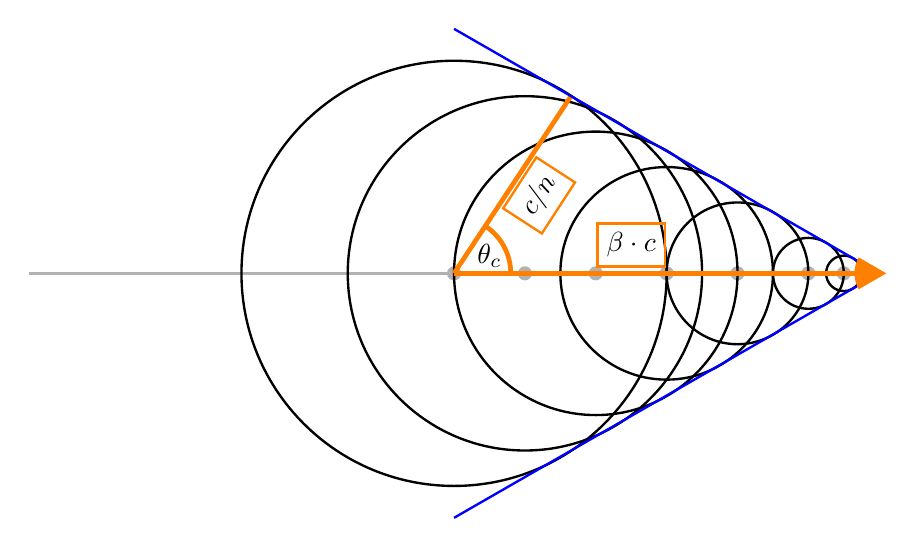
\begin{tikzpicture}[scale=0.9]
        \draw[draw=none,fill=gray!60] (8,0) circle (0.1);
        \draw[draw=none,fill=gray!60] (9,0) circle (0.1);
        \draw[draw=none,fill=gray!60] (10,0) circle (0.1);
        \draw[draw=none,fill=gray!60] (11,0) circle (0.1);
        \draw[draw=none,fill=gray!60] (12,0) circle (0.1);
        \draw[draw=none,fill=gray!60] (13,0) circle (0.1);
        \draw[draw=none,fill=gray!60] (13.5,0) circle (0.1);
        
        \draw[line width=0.3mm, gray!60] (2,0)--(14,0);
        
        \draw[line width=0.3mm] (8,0) circle (3);
        \draw[line width=0.3mm] (9,0) circle (2.5);
        \draw[line width=0.3mm] (10,0) circle (2);
        \draw[line width=0.3mm] (11,0) circle (1.5);
        \draw[line width=0.3mm] (12,0) circle (1);
        \draw[line width=0.3mm] (13,0) circle (0.5);
        \draw[line width=0.3mm] (13.5,0) circle (0.25);
        
        \draw[orange, line width=0.6mm] (8,0)--(14,0);
        \draw[orange, line width=0.6mm] (8,0)--(9.65,2.5);
        
        \draw[orange, line width=0.6mm] (8.8,0) arc (0:55:0.8cm);
        
        \draw[blue, line width=0.3mm] (8,3.45) -- (14,0);
        \draw[blue, line width=0.3mm] (8,-3.45) -- (14,0);
        
        \draw[draw=none,fill=orange] (14.1,0)-- +(210:0.45cm)arc (210:150:0.45cm) -- cycle;
        
        \node[] at (8.5,0.25) {$\theta_c$};

        \node[draw=orange,line width=0.3mm] at (10.5,0.4) {$\beta \cdot c$};
        \node[draw=orange,line width=0.3mm,, rotate=57] at (9.2,1.1) {$c/n$};
    \end{tikzpicture}
    \caption[Cherenkov light front]{Schematic formation of the Cherenkov light front (blue) produced by a charged particle traveling faster than the speed of light in the medium. The black circles are spherically emitted light and the orange arrow shows the direction of the particle.}
    \labfig{cherenkov_light_front}
\end{figure}
Typical values for the Antarctic ice are $n \approx 1.3$ and as a result $\theta_c \approx 41^\circ$ \sidecite{SEuler}.
Additionally, one can calculate the number of photons produced by a Cherenkov emitter based on the description in \sidecite{Frank_Tamm}.
For a wavelength $\lambda$ with (300\,nm < $\lambda$ < 500\,nm) 250 photons per cm are emitted assuming a very relativistic particle with $\beta \simeq 1$ \sidecite{raedel_wiebusch_cherenkov_yield}.


\subsection{Energy Losses} \labsec{energy_loss}


\subsubsection{Muons}


\subsubsection{Electromagnetic Showers}

Electromagnetic cascades are induced by electrons and positrons or photons.
All of them are either produced directly in the neutrino interactions or in interactions of secondary particles.
Photons lose energy via pair production whereas for electrons and positrons the dominant energy loss is due to bremsstrahlung.
For both cases, the interaction process happens repeatedly and an electromagnetic shower is formed when pair production and bremsstrahlung take place in turn.
Every time one of the interactions takes place, more electrons and positrons or photons are produced with smaller energy. 
This proceeds until the energy of the particles falls below the critical energy $E_c$ and the remaining energy is quickly lost.
For electrons and positrons, this happens through ionization and excitation of the surrounding atoms.
For photons, the Compton effect and the photoelectric effect become the dominant energy losses.
Electromagnetic showers are characterized by the radiation length $X_0$ at which the energy of electrons or positrons is reduced to $1/e$ of their initial energy.
For photons, $X_0$ is $7/9$ of the mean free path for pair production. For ice, the critical energy is $E_c \approx 78$\,MeV and the radiation length is $X_0 \approx 39.3$\,cm \sidecite{PhysRevD.98.030001}.


\subsubsection{Hadronic Showers}

Hadronic cascades are always produced in the neutrino interactions described in Section \refsec{neutrino_interactions}, either from the breaking nucleus or as decay products.
Similar to an electromagnetic cascade, a hadronic cascade forms as a result of the production of secondary particles from the strong interactions of hadrons with the traversed matter.
Hadronic cascades also contain an electromagnetic component, for example through the decay of neutral pions into two photons. 
The shower profile and the light emission are very dependent on the produced particle type, which leads to larger fluctuations between individual showers with the same energy.
The observed energy also varies, because energy gets lost in the hadronic binding process and muons and neutral particles produce less light and no light, respectively.
On top of that, hadrons have a higher energy threshold for Cherenkov light production, due to their higher mass.
The relative brightness of hadronic showers as compared to electromagnetic showers is given by \sidecite{LRaedel}
\begin{equation}
    F(E) = \frac{T_\mathrm{hadron}}{T_\mathrm{EM}},% = 1 - (1 - f_0)\Big(\frac{E}{E_s}\Big)^{-m}
    \labeq{relative_shower_brighness}
\end{equation}
where $T_\mathrm{hadron/EM}$ is the total track length of a hadronic/electromagnetic shower with the same energy.
The ratio $F(E)$ is always smaller than 1, but increases with energy as the electromagnetic fraction of the hadronic cascade becomes larger.
A more detailed parameterization of $F(E)$, as well as fitted values for several particle types, can be found in \sidecite{LRaedel}.


\section{Particle Signatures in IceCube} \labsec{icecube_signatures}

\subsection{Neutrinos}

\subsection{Atmospheric muons}
